%&tex
% !TEX program = xelatex
% !TeX TS-program = xelatex
% !BIB TS-program = biber
% !TeX encoding = UTF-8
% !TeX spellcheck = en_US
% !TeX root = ../thesis.tex
%% ==============================
\section{Programmable Logic Controllers}
\label{sec:plc}
%% ==============================

 
\begin{figure}
    \centering
    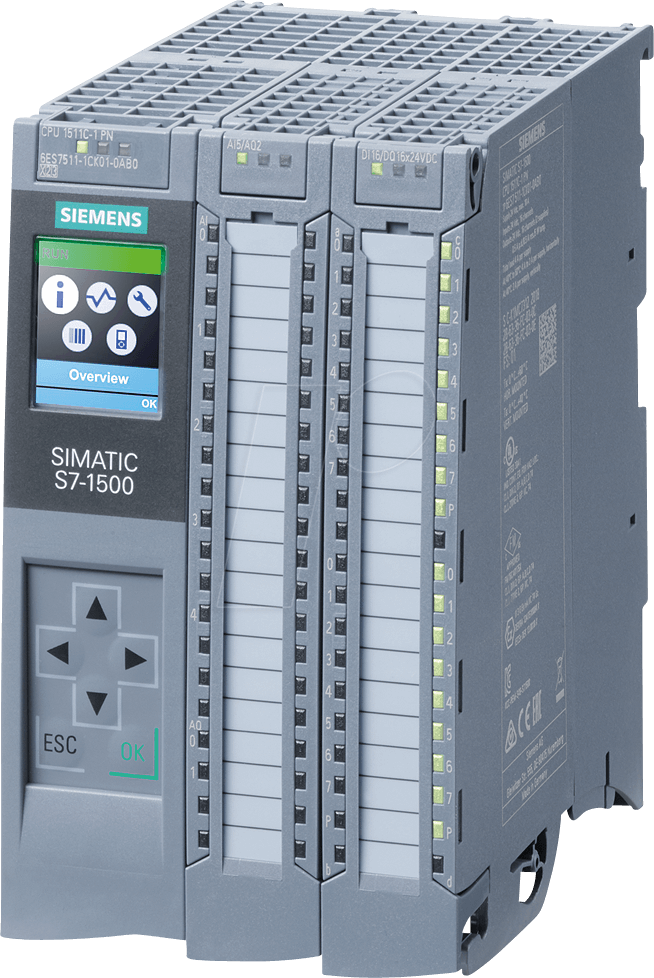
\includegraphics[width=0.5\textwidth]{Figures/simatic_s7-1500.png}
    \caption[Siemens SIMATIC S7-1500]{Siemens SIMATIC S7-1500~\acrshort{acn:plc}~\cite{Reichelt:2020}}
    \label{fig:simatic_s7}
\end{figure}

This section explains the basics of~\glspl{acn:plc} and their programming model.
They are a staple of industrial automation since the mid to late 1970's.
Major manufactures include Siemens, Rockwell Automation (Allen Bradley), Schneider Electric, Mitsubishi Electric, Omron, ABB, and General Electric~\cite{Businesswire:2016}.
An example of a modern Siemens mid range~\acrshort{acn:plc} with a attached power supply and a I/O module is shown in figure~\ref{fig:simatic_s7}.

\subsection{General}

\begin{figure}
    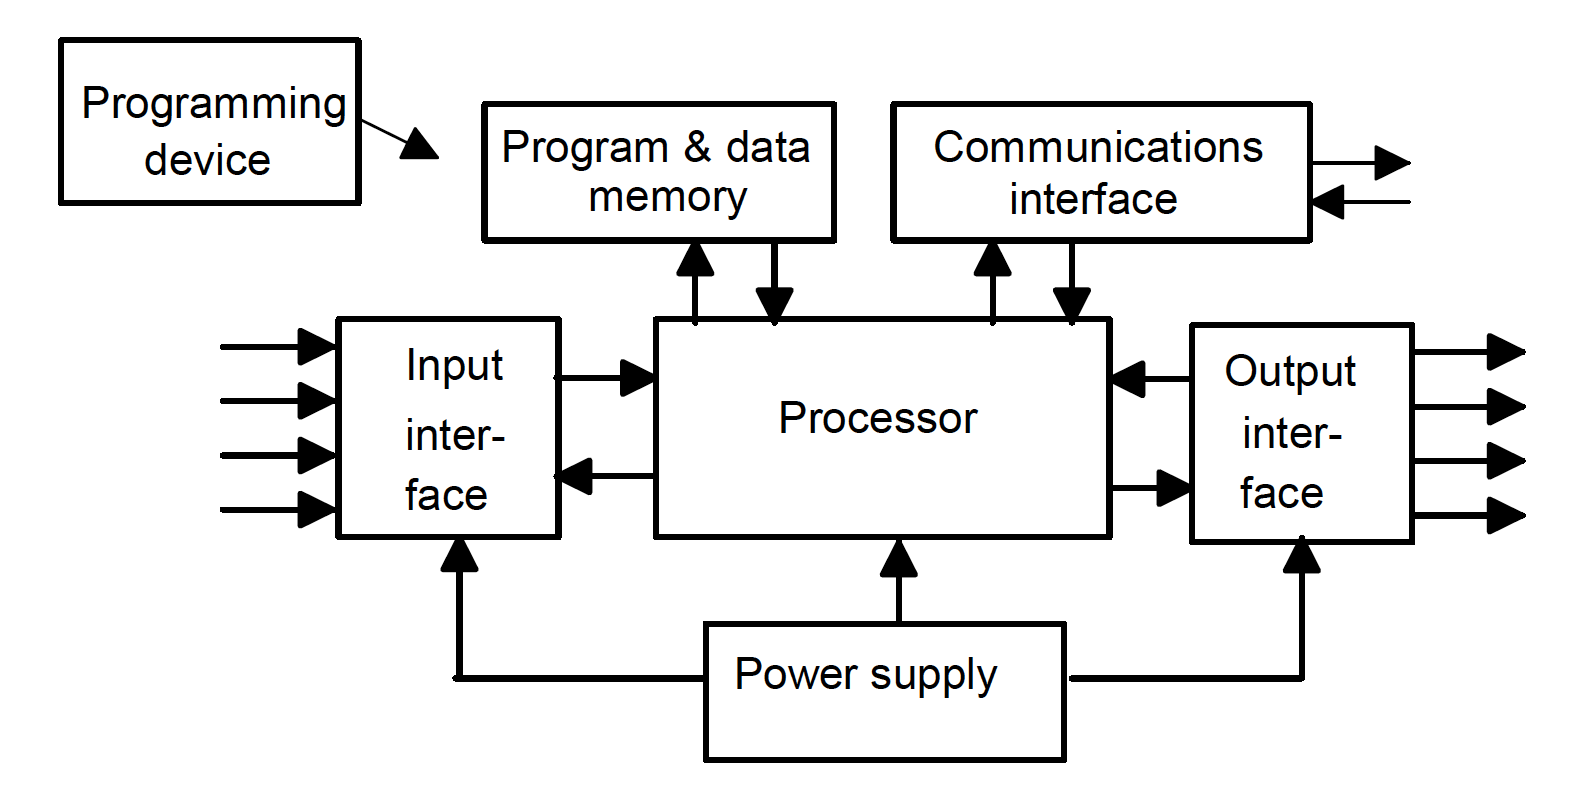
\includegraphics[width=\textwidth]{Figures/PLC_Architecture.png}
    \caption[PLC Architecture]{
       PLC Architecture~\cite[p.~4]{BOLTON200653}.
    The Input and output interfaces are either digital or analog electrical signals.
    Memories are controlled by the OS on the PLC and are programmed with a external programming device.
    Additionally PLC have a communications Interface that allows it to communicate with other controllers or devices.}
    \label{fig:plc_architecture}
\end{figure}

A~\acrfull{acn:plc} is a controller that can be programmed via simple instructions to allow the easy processing of inputs and outputs~\cite[p.~4]{BOLTON200653}.
Figure~\ref{fig:plc_architecture} shows the basic components of a~\acrshort{acn:plc}.
\acrshort{acn:plc} consist of input and output interfaces as well as a CPU that executes the current program on the inputs.
The program memory allows to change the programming of  the~\acrshort{acn:plc} without adapting any hardware components.
Additionally the data memory can be used to persist data to create stateful and complex programs.
Lastly~\acrshort{acn:plc} contain a communications interface that allows the communication with other controllers or a supervisor software.
This can for example also be used to send sensor data to a central database or implement a self management system.

A major advantage of~\acrshort{acn:plc} is that they allow for a modular design~\cite[p.~12]{BOLTON200653}, as seen with the Siemens~\acrshort{acn:plc} in figure~\ref{fig:simatic_s7}.
They are commonly assembled in a rack which allow to combine multiple modules to create a flexible configuration.
Additional hardware components, such as memory, processors, communication or I/O modules can be added with minimal effort.
This allows for standardized yet individually configurable hardware setups.
Many vendors also provide non modular single-box solutions.

Another difference between a~\acrshort{acn:plc} and a regular micro-controller is the execution semantic of a program.
\acrshort{acn:plc} programs are executed in repeating cycles.
Each cycle consists of three different phases, reading of input values into the~\acrshort{acn:ram}, execution of the program and the writing of the output variables from the~\acrshort{acn:ram}~\cite[p.~75]{BOLTON200653}.
These cycles are executed continuously during runtime, if a cycle is finished a new one starts.
The time it takes to execute a single cycle is called the cycle time.
This time depends on the processing power of the hardware, and the program complexity.
As a consequence of this execution semantic, changes to the input during a cycle are not registered until the beginning of the next cycle, and new output values are not present until the end of the current cycle.
Therefore input values have to be present for at least the cycle time to ensure they are read.
This provides a deterministic behavior of the PLC and allows for real-time capability.

\subsection{Programming with IEC 61131-3 Languages}

PLC are programmed with one of the five languages defined in the~\textit{IEC 61131-3}~\cite{Plcopen:61131-3} standard.
These languages are designed to provide a safe and well defined way of handling the inputs and outputs of the controller.
This subsection gives more details on the two most common languages used for~\acrshort{acn:plc} programming,~\acrfull{acn:ST} and the~\acrfull{acn:LD}.

\lstset{language=Pascal}
\begin{lstlisting}[caption={Example of~\gls{acn:ST} code. Source:~\cite{Wiki:ST}},label=lst:ex:st]
// PLC configuration
CONFIGURATION DefaultCfg
	VAR_GLOBAL
		// Global variable to represent a boolean.
		b_Start_Stop  : BOOL;
		// Global variable to represent a boolean.
		b_ON_OFF      : BOOL;
		// Digital   input of the PLC (Address 0.0)
		Start_Stop AT %IX0.0:BOOL;
		// Digital output of the PLC (Address 0.0). (Coil)
		ON_OFF     AT %QX0.0:BOOL;
	END_VAR

	// Schedule the main program to be executed every 20 ms
	TASK Tick(INTERVAL := t#20ms);

	PROGRAM Main WITH Tick : Monitor_Start_Stop;
END_CONFIGURATION

// Actual Program
PROGRAM Monitor_Start_Stop          
	VAR_EXTERNAL
		Start_Stop  : BOOL;
		ON_OFF      : BOOL;
	END_VAR
	VAR
		// Temporary variables for logic handling     
		ONS_Trig    : BOOL;
		Rising_ONS  : BOOL;
	END_VAR

	// Start of Logic
	// Catch the Rising Edge One Shot of the Start_Stop input
	ONS_Trig    := Start_Stop AND NOT Rising_ONS;

	// Main Logic for Run_Contact -- Toggle ON / Toggle OFF ---
	ON_OFF := (ONS_Trig AND NOT ON_OFF) OR (ON_OFF AND NOT ONS_Trig);

	// Rising One Shot logic   
	Rising_ONS := Start_Stop;
END_PROGRAM
\end{lstlisting}

\lstset{language=[x86masm]Assembler}
\begin{lstlisting}[caption={Example of~\gls{acn:IL} code. Source:~\cite{Beckhoff:IL}},label=lst:ex:il]
LD     TRUE          (*load TRUE in the accumulator*)
ANDN   BOOL1         (*execute AND with the negated value of the BOOL1 variable*)
JMPC   label         (*if the result was TRUE, then jump to the label "label"*)
LDN    BOOL2         (*save the negated value of *)
ST     ERG           (*BOOL2 in ERG*)
label:

LD     BOOL2         (*save the value of *)
ST     ERG           (*BOOL2 in ERG*)
\end{lstlisting}